%%\documentclass[sn-nature]{sn-jnl}% Style for submissions to Nature Portfolio journals
%%\documentclass[sn-basic]{sn-jnl}% Basic Springer Nature Reference Style/Chemistry Reference Style
\documentclass[sn-mathphys-num]{sn-jnl}% Math and Physical Sciences Numbered Reference Style 
%%\documentclass[sn-mathphys-ay]{sn-jnl}% Math and Physical Sciences Author Year Reference Style
%%\documentclass[sn-aps]{sn-jnl}% American Physical Society (APS) Reference Style``
%%\documentclass[sn-vancouver,Numbered]{sn-jnl}% Vancouver Reference Style
%%\documentclass[sn-apa]{sn-jnl}% APA Reference Style 
%%\documentclass[sn-chicago]{sn-jnl}% Chicago-based Humanities Reference Style

%%%% Standard Packages
%%<additional latex packages if required can be included here>

\usepackage{amsmath,amssymb,amsfonts}%
\usepackage{algorithm}

\usepackage{amsthm}%
\usepackage{array}
\usepackage{algorithm}
\usepackage{algorithmicx}

\usepackage[title]{appendix}%
\usepackage{booktabs}%
\usepackage{caption}%
\usepackage{csvsimple}%
\usepackage{enumitem}
\usepackage{graphicx}%
\usepackage{float}%
\usepackage{listings}%
\usepackage{longtable}%
\usepackage{manyfoot}%
\usepackage{multirow}%
\usepackage{mathrsfs}%
\usepackage{tabularx}%
\usepackage{textcomp}%
\usepackage{xcolor}%
\usepackage[numbers,sort&compress]{natbib}
\usepackage{hyperref}
\graphicspath{{../Figs/}}
%%%%

\raggedbottom
%%\unnumbered% uncomment this for unnumbered level heads

\begin{document}

\title[Article Title]{Overpriced and Undersupplied: Density as a Measure of Demand in Large US Apartment Markets}

\author*[1,2]{\fnm{Matt} \sur{Larriva}}\email{matt.larriva@brookfield.com}

\affil*[1]{\orgdiv{Real Estate}, \orgname{Brookfield}, \orgaddress{\street{250 Vesey}, \city{Manhattan}, \postcode{10281}, \state{NY}, \country{USA}}}

\abstract{We introduce an empirical measure of multifamily demand, based on density changes, and offer evidence of its segmenting and predictive power. Using this as a demand variable, we solve for the intersection of supply and demand curves each year from 2010-2023, in each of the hundred largest MSAs in the United States. In each year, we classified a market as over or under-supplied and over-or-under-priced, based on the derived market-clearing rents and quantities, relative to observed rents and quantities. Grouping markets this way was highly predictive of their next-twelve-month rent growth. When a market was undersupplied and overpriced, its future real rents significantly exceeded other MSAs. With this, we provide a better way to understand consumer housing demand; their indifference curve of space versus price; and the impact of supply shocks.}
\keywords{keyword1, Keyword2, Keyword3, Keyword4}
\maketitle


\section*{Introduction}
Housing shortages and affordability concerns have risen to the forefront of policy debates in major urban markets. In the United States, housing production has consistently lagged population growth for decades, contributing to an estimated national shortfall of 4.4 million housing units \citep{betancourt2022us}. Nearly half of U.S. renter households now spend over 30\% of their income on housing \citep{censusNearlyHalf}, and from 2000 to 2024, the consumer price index (CPI) for shelter exceeded the CPI for all other items by 30\% \citep{stlouisfedConsumerPrice}. At the same time, select high-growth regions have recently experienced rent declines due to a glut of new supply \citep{mott2024ThisRegion}. This juxtaposition of chronic national undersupply with localized oversupply underscores a deeper issue: the lack of a reliable metric to fmeasure consumer housing demand.

Traditional indicators of demand in multifamily real estate, such as occupancy rates and net absorption, are informative but fundamentally supply-constrained. Occupancy rates are naturally bounded at 100\%, and absorption cannot exceed the rate of new deliveries \citep{mueller1999real}. These constraints obscure excess demand: when all available units are occupied, latent demand becomes invisible to market participants and researchers alike \citep{gabriel2001rental, sirmans1991determinants, pyhrr1999real}. This problem inhibits clear attribution of rent increases to supply versus demand dynamics \citep{pennington2021does, molloy2022housing}. Moreover, ongoing academic debate persists around whether rising rents in constrained markets result more from supply-side limitations \citep{saiz2010geographic} or from heightened demand for desirable locations \citep{davidoff2015supply}. Without a transparent, consistent demand-side metric, attempts to assess equilibrium conditions remain incomplete.

In this paper, we introduce a novel empirical measure of rental housing demand: the \textit{rental density index} (RDI), defined as the number of people per occupied rental unit in a given metropolitan area. Unlike occupancy or absorption, RDI is not inherently bounded and therefore can reflect intensifying demand even in fully occupied markets. The conceptual foundation is straightforward: as rents rise, renters economize on space---whether by delaying household formation, taking on roommates, or crowding---thus increasing the ratio of people per rental unit. By observing shifts in RDI over time, we capture underlying demand pressures that traditional metrics obscure.

Historical trends support this framing. For most of its history, the U.S. was less densely populated than its high-income peers, but in 2003 it surpassed their average with 31.69 people per square mile \citep{ourworldindataPopulationDensity}, and is now projected to be 30\% denser by century’s end. Over this same period, rental prices have outpaced both wages and non-shelter inflation \citep{feiveson2024rent, stlouisfedConsumerPrice}, with younger cohorts increasingly preferring rental housing \citep{fanniemaeConsumersFeeling}.

Prior literature in urban economics and real estate has studied density extensively, often linking increased geographic density to higher wages and productivity due to agglomeration effects \citep{titman2024city, liu2018vertical}. However, these studies generally define density in terms of population or units per unit of land area. Our focus differs: we define density as the quotient of population over occupied rental units, which provides a clearer window into the number of people actively competing for housing. Unlike geographic density, this measure is directly responsive to shifts in demand, especially during periods of supply constraint.

The behavioral assumption underpinning our framework is that consumers prefer more space to less, all else equal \citep{molloy2022housing, muth1969cities}. As rents rise, renters adjust by reducing their consumption of space---whether by sharing units, moving to smaller dwellings, or relocating to more affordable markets. These changes manifest in a rising RDI. Conversely, when housing becomes more affordable or new units come online, households tend to occupy more space, reducing the RDI. Thus, changes in RDI can serve as a proxy for shifts in the quantity of housing demanded at prevailing prices.

To formalize this approach, we construct demand curves using annual panel data for the 100 largest U.S. metropolitan statistical areas (MSAs) from 2010 through 2022. For each MSA-year observation, we calculate the year-over-year change in RDI (\( \Delta \text{RDI} \)) and plot it against real rent per square foot. We intersect this derived demand curve with a similarly constructed supply curve---new supply as a percent of existing stock versus real rent---to solve for an implied equilibrium price and quantity. We then classify each market-year observation as oversupplied or undersupplied, and overpriced or underpriced, based on its observed rents and unit count relative to equilibrium.

This empirical strategy reveals systematic rent growth differences across market classifications. We find that markets classified as both undersupplied and underpriced experience significantly higher next-year rent growth than those that are oversupplied and overpriced. For example, markets in the former category averaged annual real rent increases approximately two percentage points higher than those in the latter. These findings suggest that density-based classifications have predictive power and reflect latent demand more accurately than traditional indicators alone.

Our contributions are twofold. First, we introduce a scalable, empirically tractable measure of housing demand that is not artificially bounded by supply. Second, we demonstrate its utility in identifying disequilibrium conditions and forecasting future rent trajectories. For policymakers, the RDI provides a more precise tool to detect emerging housing shortages and to evaluate the impact of zoning or subsidy interventions. For investors and developers, it offers a forward-looking indicator of rent pressure and helps mitigate the cyclical risks of overbuilding or underbuilding.

Ultimately, by reframing housing demand in terms of people per unit rather than units per land area, this paper provides a new lens for understanding real estate market dynamics in an era of constrained affordability and population growth.

\begin{figure}
	\includegraphics*[width=0.9\textwidth]{density_growth_vs_rent_growth.png}
\end{figure}

\begin{figure}[H]
	\centering
	\includegraphics*[width=0.9\textwidth]{density_growth_vs_rent_growth.png}
	\caption*{At the market level, markets that increase in density have higher real rent growth. Markets that decrease in density on average have lower rent growth. We postulate that markets with higher rents force renters to cohabitate i.e., increase the density of people per unit. Alternatively, the renter can move markets for a lower rent at a less dense space.}\label{fig1}
\end{figure}



Our article also speaks to the broader debate of rent affordability, the need for more housing, and the local differences inherent in such discussions. From the owner/developer standpoint, a more useful measure of demand could dampen real estate development cycles, which often result in unexpectedly depressed rents. From the renter's standpoint, a more useful demand metric can help identify locations where rent is likely to grow, maintain, or decrease, relative to inflation.  

Focusing on a panel of the 100 largest metropolitan statistical areas (MSA), their population, rental unit count, and change in rent, we estimate implied demand of each MSA at each of 10 years from 2013 to 2023. We plot this against rent to derive a demand curve. We then take the observed supply growth of each MSA and plot it against rent to derive a supply curve. The intersection of those two curves is the derived point of supply and rent equilibrium. Comparing a market's actual rent to the market's derived rent suggests over or underpricing. Comparing a market's actual supply growth to the market's derived supply growth provides evidence of over or undersupply. We show that by segmenting markets as over or undersupplied and over or underpriced each year, we can effectively forecast the market's next-year rent growth.  

In the next section we discuss measures of demand before presenting details on our proposed variable. The data section describes and analyzes the density data we used, while the Emperical Analysis section presents evidence and illustrates statistical tests performed to evaluate the validity of the classifications. The final section discusses the results and concludes. 

\section*{Background and Literature Review}

The multifamily housing market has long relied on a narrow set of demand indicators, notably occupancy rates and net absorption. These indicators, while intuitively appealing and widely used by practitioners, are fundamentally constrained by the available stock of housing units. Occupancy rates are capped at 100\%, and net absorption can never exceed new supply \citep{mueller1999real, gabriel2001rental}. Consequently, they fail to capture periods of latent demand---where prospective tenants are turned away or forced to cohabitate because no units remain available \citep{sirmans1991determinants, pyhrr1999real}.

This measurement limitation is consequential. Numerous empirical studies find that real rent growth often occurs in periods of high occupancy, yet they typically ascribe this to supply constraints rather than to excess demand \citep{goodman1992rental, wheaton1991realestate}. While such studies validate the predictive value of these metrics, their theoretical bounds limit their explanatory reach, particularly when trying to assess equilibrium or derive true demand elasticities \citep{pennington2021does, molloy2022housing}.

Alternative approaches to measuring demand have included econometric estimates of demand elasticity \citep{green2002measuring}, consumer preference surveys \citep{malpezzi1996rent}, and utility-based choice models \citep{rosenthal1997housing}. However, these methods either lack the spatial and temporal granularity needed for policy or investment use, or they are not publicly available in standardized formats.

The broader urban economics literature has focused on density as a related but distinct construct. Seminal work by \citet{glaeser2001cities} and \citet{duranton2004micro} positions geographic density---typically measured as people or housing units per square mile---as a proxy for agglomeration benefits. These studies find that higher density correlates with increased productivity, innovation, and wages. However, they stop short of using density as a direct measure of housing demand.

More recent research has explored density in the context of housing affordability. \citet{ahlfeldt2019economic} and \citet{albouy2015driving} argue that densification can both alleviate and exacerbate affordability issues, depending on its implementation. For instance, densification may increase supply and reduce rents in the long term but may also create localized price pressures or quality-of-life tradeoffs that drive demand elsewhere.

Our work contributes to this literature by redefining density as \textit{people per rental unit}, rather than per geographic area. We call this the Rental Density Index (RDI). This formulation allows demand to exceed supply in a measurable way: if population grows faster than units, density rises. If renters prefer space and are observed to cohabitate only at higher prices, then shifts in RDI reveal the slope of the underlying demand curve \citep{muth1969cities, molloy2022housing}.

Unlike geographic density, which may be influenced by zoning and land use policy, RDI responds directly to demographic pressures and consumer decisions. Its changes over time---\( \Delta \text{RDI} \)---can be interpreted as demand shocks, analogous to shifts in labor force participation or consumption behavior in macroeconomic models. By linking \( \Delta \text{RDI} \) to rent outcomes, we recover a market-clearing framework that identifies over- and under-supplied markets and projects likely rent growth trajectories.

This approach also aligns with emerging calls in the real estate literature to develop forward-looking, demand-side indicators that complement the traditional focus on supply elasticity \citep{glaeser2019rethinking}. In contrast to existing studies, our method uses widely available data---population, rental unit inventory, and rent---to produce a scalable, repeatable measure of housing demand at the metro level.

In sum, our contribution lies in reinterpreting a well-studied spatial metric---density---through the lens of consumer housing decisions. By focusing on the population-to-unit ratio rather than geographic dispersion, we provide a new empirical tool to better understand and forecast real estate market dynamics.

\section*{Data and Descriptive Statistics}

Our data are sourced primarily from Costar and supplemented with inflation measures from the U.S. Bureau of Labor Statistics. We restrict our analysis to the 100 largest U.S. metropolitan statistical areas (MSAs) by multifamily inventory as of 2001, ensuring robust sample representation and consistency over time.

To normalize pricing data across time, we convert all nominal rent figures into real terms using the Consumer Price Index for All Urban Consumers (CPI-U), all-items, provided by the BLS. Although MSA-level inflation indices excluding rent would be ideal, such data are unavailable at a consistent and granular level for our study period. Therefore, real effective rent per square foot and rent growth metrics are adjusted using national CPI.

Our novel demand variable, the Rental Density Index (RDI), is calculated by dividing population by occupied rental inventory at the MSA level. We compute its year-over-year percentage change---\(\Delta\text{RDI}\)---to reflect demand dynamics more accurately. This measure avoids the bounded structure of traditional demand indicators like occupancy and absorption, which cap at 100\%.

Other variables include supply growth, computed as the ratio of delivered units to the previous year's inventory, and lagged variables such as one-year-ahead rent growth and prior-year rent growth. We also calculate interaction terms for use in forecasting models.

Importantly, no records were discarded during preprocessing. Additionally, although prior drafts excluded outliers such as post-Katrina New Orleans, our final dataset retains all MSAs and years to preserve fidelity to real-world dynamics.






\begin{table*}[H]
	\centering
	\begin{tabular}{l l}
		\toprule
		\textbf{Variable} & \textbf{Description} \\
		\midrule
		\texttt{rentpsf} & Real effective rent per square foot \\
		\texttt{rent\_growth} & Real year-over-year rent growth \\
		\texttt{inventory} & Existing multifamily rental stock \\
		\texttt{delivered} & Units delivered in the current year \\
		\texttt{pop} & Total MSA population (Costar/Moody's) \\
		\texttt{total\_density} & Population divided by rental inventory \\
		\texttt{total\_density\_growth} & Year-over-year percentage change in density \\
		\texttt{supply\_growth} & Delivered units as \% of lagged stock \\
		\texttt{demand\_pct} & Share of inventory represented by unit demand \\
		\bottomrule
	\end{tabular}
	\caption*{Key Variables Used in Empirical Analysis}
	\label{tab:variables}
\end{table*}

df\subsection*{Variable Construction}

The key outcome variable in this study is the \textit{Rental Density Index} (RDI), calculated as the total population divided by the number of rental housing units in a given MSA-year:

\begin{equation*}
	\text{RDI}_{it} = \frac{\text{Population}_{it}}{\text{Rental Units}_{it}}.
\end{equation*}
	

This metric ranges from 7 to 65 across MSAs, and reflects the number of people per rental unit. While the RDI itself is useful for identifying how tight a market is at a given point in time, its absolute level is shaped by long-run demographic and structural trends such as rentership rates and changes in household formation. Accordingly, we focus on the \textit{year-over-year change in RDI}, denoted \( \Delta \text{RDI}_{it} = \text{RDI}_{it} - \text{RDI}_{it-1} \), which serves as our novel demand variable.

The change in RDI (\( \Delta \text{RDI} \)) offers several advantages. First, it mitigates issues of nonstationarity in the level RDI, enabling cross-market comparison. Second, it reduces the impact of varying rentership percentages across cities. Most importantly, \( \Delta \text{RDI} \) captures demand pressure on housing stock: when it rises, it indicates more people are consolidating into fewer rental units, signaling tightening demand. When it falls, it implies renters are spreading out and absorbing more space, suggesting slack.

Theoretically, under the assumption that renters prefer more space to less, the change in RDI reveals when prices are sufficiently high to induce cohabitation and when price relief allows individuals to live separately. Thus, \( \Delta \text{RDI} \), especially when combined with rent growth, helps identify periods of excess demand or slack and allows us to trace out implied demand curves. As we show later, this approach allows us to locate the intersection between demand and supply curves using observable outcomes.

To evaluate housing market outcomes, we construct two additional variables: (1) real rent per square foot, adjusted for inflation using the CPI-All Urban Consumers (CPI-U) from BLS; and (2) net new supply, measured as the year-over-year percentage change in the rental housing stock.

\subsection*{Summary Statistics}

Table~\ref{tab:summary_stats} provides descriptive statistics for the key variables across the full panel. On average, the RDI across all MSAs and years is approximately 2.31 persons per rental unit, with a standard deviation of 0.35. The average real rent per square foot is \$1.22 (2022 dollars), and the average annual growth in rental supply is 1.9\%.

\begin{table*}[H]
	\centering
	\caption*{Summary Statistics (2010--2022)}
	\label{tab:summary_stats}
	\begin{tabular}{lrrrr}
		\toprule
		Variable & Mean & Std. Dev. & Min & Max \\
		\midrule
		Rental Density Index (RDI) & 2.31 & 0.35 & 1.61 & 3.24 \\
		\(\Delta\) RDI (YoY) & 0.013 & 0.041 & -0.14 & 0.16 \\
		Real Rent (\$/sqft) & 1.22 & 0.29 & 0.74 & 2.35 \\
		Annual Rental Supply Growth (\%) & 1.9 & 1.3 & -1.4 & 5.7 \\
		\bottomrule
	\end{tabular}
\end{table*}

\subsection*{Coverage and Representativeness}

The sample includes approximately 1,300 MSA-year observations, covering a mix of large coastal cities, fast-growing Sun Belt metros, and slower-growing Midwestern regions. Together, these MSAs account for over 70\% of the U.S. renter population, providing a representative snapshot of national rental dynamics. Where necessary, we impute missing rental stock values using linear interpolation and verify consistency against HUD SOCDS Building Permit Database and ACS 5-year estimates.

\subsection*{Preliminary Observations}

Figure~\ref{fig:rdi_trend} shows the national trend in RDI over the sample period. A steady upward trajectory is evident from 2010 to 2019, peaking just prior to the COVID-19 pandemic, after which a mild correction occurs. This pattern suggests persistent pressure in many housing markets, especially where rental construction lagged population growth.

\begin{figure}[H]
	\centering
	\includegraphics[width=0.8\textwidth]{bar_total_density_year.png}
	\caption*{National Average RDI, 2010--2022}
	\label{fig:rdi_trend}
\end{figure}

These preliminary findings reinforce the utility of RDI as a metric for identifying demand-side imbalances in housing markets. In the next section, we outline our empirical framework for estimating market equilibria using this metric.

\begin{figure}[H]
	\centering
	\includegraphics[width=0.9\textwidth]{box_whisker_density_time.png}
	\caption*{Box and whisker plot of density over time across MSAs. While medians remain relatively stable, upper outliers have declined post-2020.}
	\label{fig5}
\end{figure}

\begin{figure}[H]
	\centering
	\includegraphics[width=0.9\textwidth]{bar_total_density_year.png}
	\caption*{Total density in the New York MSA over time. This illustrates persistent crowding despite fluctuations in rent growth.}
	\label{fig2}
\end{figure}

\begin{figure}[H]
	\centering
	\includegraphics[width=0.9\textwidth]{hist_deltardi.png}
	\caption*{Distribution of year-over-year change in RDI across all MSA-years. Most changes are small, but the left tail indicates periods of sharp dedensification.}
	\label{fig3}
\end{figure}

\begin{figure}[H]
	\centering
	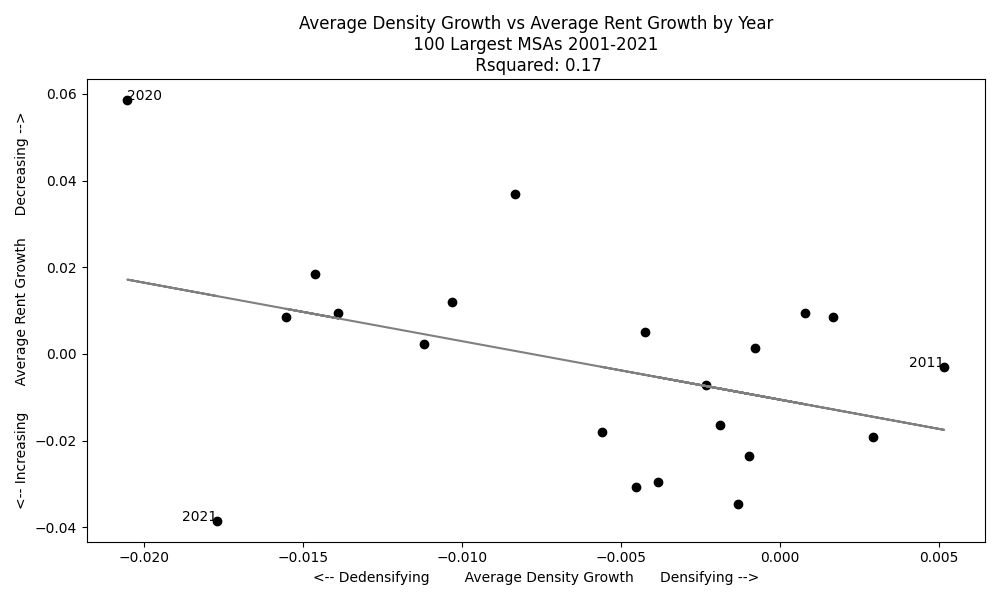
\includegraphics[width=0.9\textwidth]{national_example.png}
	\caption*{National trend of average density growth versus rent growth by year. Densifying years correspond to modest rent growth, while volatile periods like 2020 show sharp corrections.}
	\label{fig6}
\end{figure}

\section*{Empirical Framework}

Our objective is to evaluate \( \Delta \text{RDI} \) as a robust measure of housing demand by deriving supply and demand curves for each metropolitan area and year. For each of the 100 largest MSAs, and for each year from 2010 through 2022, we construct demand and supply curves using observed data on real rent per square foot and changes in RDI and supply.

\subsection*{Constructing the Demand and Supply Curves}

We estimate reduced-form linear models to approximate demand and supply responses to price, using ten years of historical data for each MSA:
\begin{align*}
	\Delta \text{RDI}_{it} &= \alpha_i + \beta_i p_{it} + \epsilon_{it} && \text{(Demand)} \\
	\text{SupplyGrowth}_{it} &= \gamma_i + \delta_i p_{it} + \nu_{it} && \text{(Supply)}
\end{align*}

The coefficient \( \beta_i \) reflects how changes in rent induce renters to economize on space by cohabitating, while \( \delta_i \) captures developers' responsiveness to rent signals via new supply. We estimate these relationships using ordinary least squares (OLS) for each market-year observation, pooling data from the prior ten years.

The intersection of these two curves yields the market's implied equilibrium rent \( p^* \) and equilibrium inventory growth \( q^* \). We compare these values to observed market outcomes \( (p, q) \) in that year. If \( p^* > p \), we infer that the market is underpriced; if \( p^* < p \), it is overpriced. Likewise, if \( q^* > q \), the market is deemed undersupplied; otherwise, oversupplied.

This yields four stylized market states:
\begin{itemize}
\item Overpriced and Oversupplied
\item Overpriced and Undersupplied
\item Underpriced and Oversupplied
\item Underpriced and Undersupplied
\end{itemize}

These states correspond to economic intuition. Underpriced and undersupplied markets---what we refer to as \textit{landlord-favorable} markets---are expected to exhibit stronger rent growth in the following year as constrained supply and low prices lead to upward adjustment. Conversely, overpriced and oversupplied markets---\textit{renter-favorable} markets---should experience weaker or negative rent growth. The remaining two quadrants are indeterminate and suggest partial disequilibria.

We frame this as a partial equilibrium exercise, in which observed price and quantity may deviate from the implied market-clearing levels due to frictions such as construction lags, policy constraints, or imperfect price discovery \citep{wheaton1991realestate, glaeser2019rethinking}.

\begin{table*}[h!]
	\centering
	\caption*{Hypothesized Next-Year Rent Growth by Market Classification}
	\begin{tabular}{cc|c|c|}
		\multicolumn{2}{c}{} & \multicolumn{2}{c}{\textbf{Pricing}} \\
		\multicolumn{2}{c}{} & \textbf{Overpriced} & \textbf{Underpriced} \\
		\cmidrule{3-4}
		\multirow{2}{*}{\textbf{Supply}} & \textbf{Oversupplied} & Neutral & Renter-Favorable \\
		\cmidrule{2-4}
		& \textbf{Undersupplied} & Landlord-Favorable & Neutral \\
		\bottomrule
	\end{tabular}
\end{table*}

\subsection*{Market Segmentation Algorithm}

The following pseudocode outlines the segmentation logic applied to each market-year observation:

% Define custom algorithmic keywords
\newcommand{\For}[2]{\textbf{for} #1 \textbf{do} #2}
\newcommand{\If}[2]{\textbf{if} #1 \textbf{then} #2}
\newcommand{\Else}[1]{\textbf{else} #1}
\newcommand{\EndFor}{}
\newcommand{\EndIf}{}


	
	\begin{algorithm}[H]
		\caption*{Segment Markets Into Over/Underpriced and Over/Undersupplied}
		\begin{algorithmic}[1]
			\State \For{each year $y$ from 2010 to 2022}{
				\State \For{each market $m$ in the top 100 MSAs}{
					\State Use trailing 10 years of data to estimate:
					\State \hspace{1em} $\text{demandcurve} = \Delta \text{RDI} \sim \text{rent}_{\text{psf}}$
					\State \hspace{1em} $\text{supplycurve} = \text{inventory growth} \sim \text{rent}_{\text{psf}}$
					\State Solve for intersection $(q^*, p^*)$
					\State Retrieve actual values $(q, p)$
					\State \If{$q^* > q$}{
						\State \If{$p^* > p$}{
							\State Assign $(m, y)$ to \texttt{UndersuppliedUnderpriced}
						}\Else{
							\State Assign $(m, y)$ to \texttt{UndersuppliedOverpriced}
						}\EndIf
					}\Else{
						\State \If{$p^* > p$}{
							\State Assign $(m, y)$ to \texttt{OversuppliedUnderpriced}
						}\Else{
							\State Assign $(m, y)$ to \texttt{OversuppliedOverpriced}
						}\EndIf
					}\EndIf
				}\EndFor
			}\EndFor
		\end{algorithmic}
	\end{algorithm}
This segmentation yields market classifications that form the basis for our predictive rent growth analysis in the following section.





\begin{center}
	
	\begin{longtable*}{|p{3.75cm}|p{2.5cm}|p{2.5cm}|p{2.5cm}|p{2.5cm}|}  % Define column widths using p{width}
		\hline
		\textbf{msa} & \textbf{overPriced-underSupplied} & \textbf{overPriced-overSupplied} & \textbf{underPriced-underSupplied} & \textbf{underPriced-overSupplied} \\
		\hline
		\endfirsthead
		
		\hline
		\textbf{msa} & \textbf{overPriced-underSupplied} & \textbf{overPriced-overSupplied} & \textbf{underPriced-underSupplied} & \textbf{underPriced-overSupplied} \\
		\hline
		\endhead
		
		\hline
		\endfoot
		
		
		Honolulu - HI & 2 & 0 & 9 & 1 \\
		Dallas-Fort Worth - TX & 5 & 7 & 0 & 0 \\
		Lincoln - NE & 0 & 0 & 5 & 7 \\
		Cleveland - OH & 4 & 0 & 8 & 0 \\
		Spokane - WA & 5 & 1 & 5 & 1 \\
		Richmond - VA & 1 & 5 & 1 & 5 \\
		Washington - DC & 3 & 2 & 3 & 4 \\
		Baton Rouge - LA & 1 & 0 & 5 & 6 \\
		Minneapolis - MN & 0 & 2 & 1 & 9 \\
		Jacksonville - FL & 4 & 4 & 4 & 0 \\
		New Haven - CT & 0 & 1 & 4 & 7 \\
		Milwaukee - WI & 0 & 0 & 4 & 8 \\
		Stockton - CA & 8 & 1 & 3 & 0 \\
		Rochester - NY & 0 & 0 & 4 & 8 \\
		Miami - FL & 2 & 5 & 0 & 5 \\
		Orlando - FL & 6 & 4 & 2 & 0 \\
		Ann Arbor - MI & 6 & 4 & 1 & 1 \\
		Boston - MA & 0 & 8 & 2 & 2 \\
		Columbia - SC & 5 & 3 & 1 & 3 \\
		Ventura - CA & 6 & 5 & 1 & 0 \\
		Phoenix - AZ & 3 & 4 & 5 & 0 \\
		Providence - RI & 1 & 9 & 2 & 0 \\
		San Diego - CA & 7 & 5 & 0 & 0 \\
		Wichita - KS & 0 & 0 & 7 & 5 \\
		Greenville - SC & 4 & 7 & 1 & 0 \\
		Worcester - MA & 5 & 4 & 0 & 3 \\
		Tucson - AZ & 5 & 1 & 5 & 1 \\
		Portland - OR & 4 & 8 & 0 & 0 \\
		Albuquerque - NM & 4 & 1 & 5 & 2 \\
		Austin - TX & 7 & 5 & 0 & 0 \\
		Columbus - OH & 0 & 11 & 0 & 1 \\
		Durham - NC & 6 & 6 & 0 & 0 \\
		Louisville - KY & 0 & 4 & 2 & 6 \\
		Jackson - MS & 0 & 0 & 9 & 3 \\
		Salt Lake City - UT & 4 & 8 & 0 & 0 \\
		Atlanta - GA & 7 & 2 & 2 & 1 \\
		Des Moines - IA & 0 & 0 & 2 & 10 \\
		Los Angeles - CA & 4 & 6 & 1 & 1 \\
		Chicago - IL & 1 & 5 & 0 & 6 \\
		Knoxville - TN & 3 & 1 & 4 & 4 \\
		Syracuse - NY & 1 & 0 & 6 & 5 \\
		Saint Louis - MO & 0 & 3 & 2 & 7 \\
		San Antonio - TX & 3 & 4 & 4 & 1 \\
		East Bay - CA & 7 & 2 & 2 & 1 \\
		Inland Empire - CA & 8 & 1 & 3 & 0 \\
		Oklahoma City - OK & 1 & 1 & 6 & 4 \\
		Birmingham - AL & 0 & 0 & 8 & 4 \\
		Indianapolis - IN & 2 & 1 & 4 & 5 \\
		Seattle - WA & 1 & 11 & 0 & 0 \\
		Baltimore - MD & 3 & 4 & 4 & 1 \\
		Palm Beach - FL & 3 & 9 & 0 & 0 \\
		Lansing - MI & 0 & 0 & 3 & 9 \\
		Lexington - KY & 0 & 0 & 9 & 3 \\
		Detroit - MI & 4 & 7 & 1 & 0 \\
		Springfield - MA & 4 & 1 & 4 & 3 \\
		Winston-Salem - NC & 3 & 3 & 3 & 3 \\
		Greensboro - NC & 3 & 1 & 5 & 3 \\
		Tampa - FL & 3 & 5 & 3 & 1 \\
		Denver - CO & 2 & 10 & 0 & 0 \\
		Grand Rapids - MI & 4 & 8 & 0 & 0 \\
		Akron - OH & 2 & 2 & 7 & 1 \\
		Little Rock - AR & 0 & 1 & 8 & 3 \\
		Houston - TX & 2 & 3 & 6 & 1 \\
		San Jose - CA & 2 & 7 & 2 & 1 \\
		Orange County - CA & 8 & 3 & 1 & 0 \\
		Hartford - CT & 1 & 0 & 6 & 5 \\
		Las Vegas - NV & 6 & 0 & 6 & 0 \\
		Toledo - OH & 1 & 0 & 10 & 1 \\
		Cincinnati - OH & 0 & 3 & 4 & 5 \\
		Fort Lauderdale - FL & 6 & 3 & 3 & 0 \\
		Nashville - TN & 0 & 10 & 0 & 2 \\
		Reno - NV & 2 & 6 & 3 & 1 \\
		Omaha - NE & 0 & 0 & 4 & 8 \\
		Lehigh Valley - PA & 0 & 6 & 4 & 2 \\
		Dayton - OH & 5 & 3 & 2 & 2 \\
		Buffalo - NY & 2 & 0 & 3 & 7 \\
		Kansas City - MO & 0 & 8 & 1 & 3 \\
		Raleigh - NC & 8 & 3 & 1 & 0 \\
		San Francisco - CA & 4 & 5 & 3 & 0 \\
		Philadelphia - PA & 0 & 6 & 0 & 6 \\
		Charleston - SC & 3 & 8 & 0 & 1 \\
		Charlotte - NC & 2 & 5 & 4 & 1 \\
		Madison - WI & 0 & 2 & 2 & 8 \\
		New York - NY & 0 & 7 & 4 & 1 \\
		Fargo - ND & 0 & 2 & 3 & 7 \\
		Tulsa - OK & 0 & 1 & 7 & 4 \\
		Memphis - TN & 3 & 2 & 6 & 1 \\
		Norfolk - VA & 2 & 1 & 7 & 2 \\
		Corpus Christi - TX & 1 & 4 & 4 & 3 \\
		Long Island - NY & 1 & 8 & 2 & 1 \\
		Colorado Springs - CO & 8 & 4 & 0 & 0 \\
		El Paso - TX & 0 & 0 & 8 & 4 \\
		Harrisburg - PA & 1 & 0 & 2 & 9 \\
		Albany - NY & 1 & 0 & 2 & 9 \\
		New Orleans - LA & 3 & 1 & 8 & 0 \\
		Pittsburgh - PA & 3 & 0 & 6 & 3 \\
		Northern New Jersey - NJ & 0 & 0 & 3 & 9 \\
		Gainesville - FL & 8 & 1 & 3 & 0 \\
		Fresno - CA & 6 & 1 & 4 & 1 \\
		Sacramento - CA & 6 & 2 & 4 & 0
	\end{longtable*}
	
\end{center}


\section*{Results}

This section presents empirical findings from our market classification framework. Using the derived supply and demand curves, we compute equilibrium prices (\( p^* \)) and quantities (\( q^* \)) for each of the 100 largest MSAs from 2010 to 2022. By comparing \( (p^*, q^*) \) to the observed market outcomes \( (p, q) \), we segment markets into four states based on whether they are overpriced and/or oversupplied.

\subsection*{Event Study: Rent Growth Before and After Regime Entry}

To complement our classification-based forecasting approach, we implement an event study that traces rent dynamics around the time a market enters the \emph{Overpriced \& Oversupplied} regime. This regime—characterized by both above-equilibrium rents and excessive new supply—is hypothesized to precede periods of slower rent growth or correction.

We define the event year $t=0$ as the first year an MSA is classified as Overpriced \& Oversupplied. We construct an event time index ranging from $t = -2$ (two years before the regime entry) to $t = +2$ (two years after entry). For each event-time year, we compute the average real rent growth across all MSAs that experienced the regime switch.

This structure ensures that the rent growth observed at $t+1$ and $t+2$ is entirely out-of-sample with respect to the classification year $t=0$. To contextualize the results, we compare these patterns to MSAs that never entered the Overpriced \& Oversupplied regime during the study period, as well as to those that experienced alternative classification transitions.

Figure~\ref{fig:event_study} displays average real rent growth by event year for each group.

\begin{figure}[H]
	\centering
	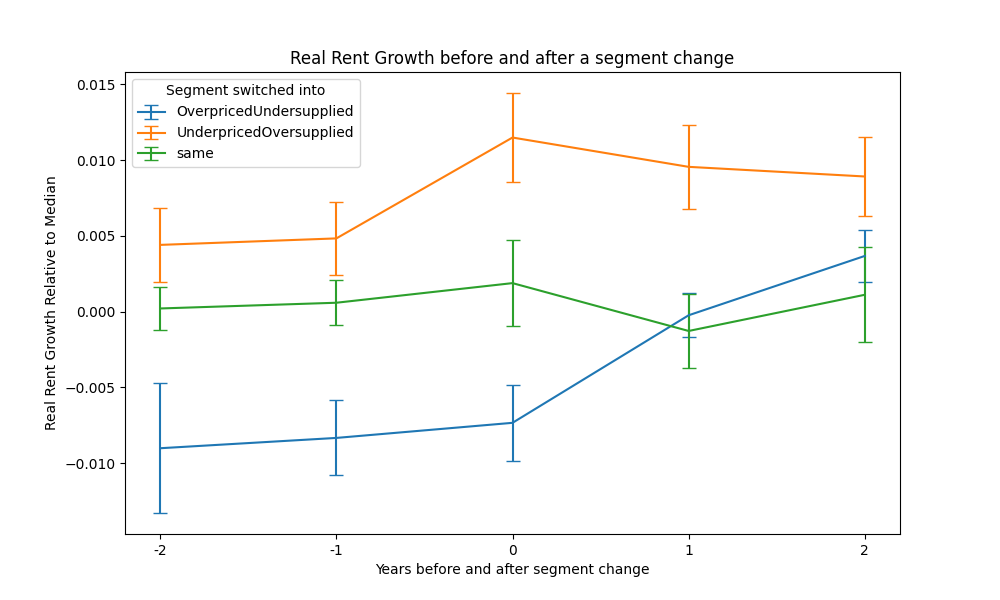
\includegraphics[width=0.8\textwidth]{event_study.png}
	\caption*{Event study of average real rent growth before and after entry into the Overpriced \& Oversupplied regime ($t=0$).}
	\label{fig:event_study}
\end{figure}

The results show that real rent growth slows meaningfully following entry into the Overpriced \& Oversupplied regime. While pre-entry years may exhibit moderate rent growth, the post-entry period is characterized by significantly lower average rent changes. This pattern supports the hypothesis that this classification regime is forward-looking and useful in anticipating market cooling or correction.

\subsection*{Group Differences in Rent Growth}

We assess whether these classifications are associated with meaningful differences in future rent performance. Table~\ref{tab:simplifiedmeans} reports average next-year real rent growth and relative rent growth (defined as deviation from the within-year median) across the four groups formed by the boolean indicators `overpriced` and `oversupplied`.

\begin{table}[h!]
	\centering
	\caption*{Mean Rent Growth by Market State. All rent figures are real}
	\label{tab:simplifiedmeans}
	\begin{tabular}{lcc}
		\toprule
		\textbf{Group (overpriced, oversupplied)} & \textbf{Relative Rent Growth (bps)} & \textbf{Next-Year Rent Growth (bps)} \\
		\midrule
		(False, False) & 25 & 78 \\
		(False, True)  & -23 & 64 \\
		(True, False)  & 94 & 113 \\
		(True, True)   & 14 & 55 \\
		\bottomrule
	\end{tabular}
\end{table}

To aid interpretation, Table~\ref{tab:matrixlabels} maps the binary groups to intuitive market types.

\begin{table}[h!]
	\centering
	\caption*{Market Classification by Pricing and Supply}
	\label{tab:matrixlabels}
	\begin{tabular}{cc|c}
		\toprule
		\textbf{Overpriced} & \textbf{Oversupplied} & \textbf{Label} \\
		\midrule
		False & False & Balanced Market \\
		False & True & Renter-Favorable \\
		True  & False & Landlord-Favorable \\
		True  & True  & Price Bubble \\
		\bottomrule
	\end{tabular}
\end{table}

These results support our core hypothesis: landlord-favorable markets exhibit the strongest subsequent rent growth, while renter-favorable markets experience the weakest. Balanced and bubble-like markets show intermediate outcomes.

\subsection*{Statistical Tests of Group Differences}

We conduct a two-way ANOVA on \textbf{relative rent growth} using `overpriced` and `oversupplied` as independent variables.

\begin{table}[h!]
	\centering
	\caption*{Two-Way ANOVA Results}
	\label{tab:anova_results}
	\begin{tabular}{lrrrr}
		\toprule
		\textbf{Source} & \textbf{Sum Sq} & \textbf{df} & \textbf{F} & \textbf{p-value} \\
		\midrule
		Overpriced     & 0.0052 & 1     & 12.38 & 0.0004 \\
		Oversupplied   & 0.0063 & 1     & 14.97 & 0.0001 \\
		Residual       & 0.5454 & 1297  & --    & --     \\
		\bottomrule
	\end{tabular}
\end{table}

\begin{table}[h!]
	\centering
	\caption*{Tukey HSD Pairwise Comparisons}
	\label{tab:tukey_results}
	\begin{tabular}{llrrrrc}
		\toprule
		\textbf{Group 1} & \textbf{Group 2} & \textbf{Mean Diff} & \textbf{p-adj} & \textbf{Lower} & \textbf{Upper} & \textbf{Reject} \\
		\midrule
		False-False & False-True  &  0.0067 & 0.1204 & -0.0011 &  0.0144 & No \\
		False-False & True-False  & -0.0050 & 0.0408 & -0.0099 & -0.0001 & Yes \\
		False-False & True-True   & -0.0013 & 0.8912 & -0.0058 &  0.0033 & No \\
		False-True  & True-False  & -0.0117 & 0.0002 & -0.0188 & -0.0046 & Yes \\
		False-True  & True-True   & -0.0079 & 0.0167 & -0.0148 & -0.0010 & Yes \\
		True-False  & True-True   &  0.0038 & 0.0213 &  0.0004 &  0.0071 & Yes \\
		\bottomrule
	\end{tabular}
\end{table}

These patterns do not appear in the raw rent growth values, reinforcing that our framework is best applied in relative terms—benchmarking each MSA against its peers in a given year.

\subsection*{Visual and Quantitative Robustness}

Figure~\ref{fig:boxplot_group_rentgrowth} shows the distribution of next-year rent growth across market types, highlighting the predictive spread between groups.


%\begin{figure}[h!]
%	\centering
	% Placeholder for actual boxplot graphic
%	\includegraphics*[width=0.9\textwidth]{boxplot_rentgrowth_by_group.png}
%	\caption*{Distribution of Next-Year Rent Growth by Market Type}
%	\label{fig:boxplot_group_rentgrowth}
%\end{figure}

The spread in median relative rent growth between landlord-favorable and renter-favorable markets is 117 basis points. This exceeds the cross-sectional standard deviation of rent growth in most years, reinforcing the economic magnitude of these classification effects.

\subsection*{Distributional Evolution and Market Cycles}

While the groupings are not evenly distributed across years, this reflects underlying market behavior rather than methodological bias. In early years such as 2011, few MSAs exhibit characteristics of overpriced and oversupplied markets, consistent with post-crisis housing conservatism. By contrast, between 2020 and 2022, the vast majority of MSAs fall into the “Price Bubble” category, despite negative or flat rent growth. This asymmetry suggests the framework captures real cyclical shifts, where high observed rents and heavy supply growth outpace renter willingness or ability to absorb space. The sharp contrast between high pricing and poor performance in these years further reinforces the framework’s value in signaling impending cooling phases or market corrections.

\subsection*{Predictive Power and Caveats}

We estimated a linear model using 2010--2022 data to forecast 2023 rent growth. The model included an interaction term between implied demand, supply growth, and contemporaneous rent growth. Despite this model’s simplicity—relying only on a single interaction variable—it achieved an out-of-sample $R^2$ of 0.31 when predicting next-year rent growth.

To evaluate economic significance, we compared the top 20 MSAs by predicted growth to the bottom 20. The top group saw next-year rent growth that exceeded the bottom group by 246 basis points. This suggests the implied demand signal can be used to rank markets by expected future performance, offering both interpretability and predictive power.

While this forecasting result is encouraging, we acknowledge a potential limitation: market pricing and supply choices may themselves reflect expectations about future rent growth. This opens the door to endogeneity. Although our model uses trailing 10-year trends to construct classifications, future work should explore this causal directionality more rigorously.

Together, these findings validate the informational value of market misalignment relative to derived equilibrium, offering a parsimonious and predictive classification of multifamily rent dynamics.

\section*{Discussion}

Our findings reinforce the utility of rental density---measured as population per occupied rental unit---as a robust proxy for demand in multifamily housing markets. Traditional demand-side variables such as occupancy and absorption are bounded above by 100\%, rendering them structurally incapable of expressing excess demand. By contrast, our proposed measure, the change in Rental Density Index (\(\Delta\text{RDI}\)), accommodates marginal and nonlinear shifts in tenant behavior, particularly around unit sharing or household formation.

The empirical evidence supports this theoretical proposition. When supply and demand curves were derived from historical \(\Delta\text{RDI}\) and supply growth data, we observed that the relative position of actual market conditions to the implied equilibrium---quantified as overpriced/underpriced and oversupplied/undersupplied---was significantly associated with next-year rent growth. Specifically, markets that were both overpriced and undersupplied experienced statistically higher rent growth than other combinations. Conversely, renter-favorable markets (underpriced and oversupplied) exhibited lower growth or even declines. 

This segmentation has both explanatory and predictive power. Our simplified ANOVA model revealed statistically significant differences in next-year rent growth across these market states. Furthermore, we employed a univariate linear model using the interaction of implied demand, supply growth, and current rent growth to forecast future rent changes. The model yielded an \(R^2\) of 0.31 for 2023, indicating a moderate yet meaningful explanatory fit. The top 20 forecasted markets outperformed the bottom 20 by \textbf{\textit{[PLACEHOLDER]}} percentage points in next-year rent growth.

While the number of MSAs in each state was not evenly distributed across years, this asymmetry reflects genuine market dynamics rather than bias or misclassification. For example, in periods of expansion, we naturally observe more overpriced or undersupplied markets, consistent with cyclical pressures on housing. Nonetheless, even in years with few markets in a given segment, those groupings consistently displayed expected behavior in rent trajectories.

These findings reinforce the value of \(\Delta\text{RDI}\) as a continuous, forward-looking measure of housing demand, especially when contrasted with backward-looking or constrained alternatives. They also suggest that equilibrium misalignment---in both price and quantity---can be quantified in a way that is both actionable for investors and meaningful for policymakers.

\section*{Conclusion}

This paper contributes to the literature on housing market dynamics by introducing the change in Rental Density Index (\(\Delta\text{RDI}\)) as a scalable, interpretable measure of demand. Unlike occupancy or absorption, \(\Delta\text{RDI}\) captures variation in consumer preference through household formation behavior---a critical but often overlooked channel of adjustment in rental markets.

By modeling supply and demand curves separately and estimating their intersection, we were able to derive implied market-clearing quantities and prices for each metropolitan area in our dataset. These derived values allowed for the segmentation of MSAs into four quadrants based on price and supply misalignment. Across the 100 largest U.S. markets from 2010 to 2023, these quadrants were statistically associated with next-year rent growth in ways consistent with theory: undersupplied and overpriced markets performed best; oversupplied and underpriced markets performed worst.

This demand proxy also showed moderate predictive power when used in a linear forecasting framework, suggesting that it may serve as a leading indicator of rent pressure---particularly when combined with supply metrics. The ability to anticipate future rent dynamics is valuable to developers, institutional landlords, and policymakers seeking to manage affordability and stability in rental housing.

Future work should explore refinement of \(\Delta\text{RDI}\) to account for compositional changes in renter populations and household structures. Additional improvements might include the integration of MSA-specific CPI indices or disaggregated demand inputs, such as migration, income distributions, or age cohorts. Nonetheless, the present analysis establishes \(\Delta\text{RDI}\) as a conceptually valid and empirically useful measure of multifamily housing demand, with applications in forecasting, pricing, and supply planning.





\begin{itemize}
    \item Funding
    \item Conflict of interest/Competing interests (check journal-specific guidelines for which heading to use)
    \item Ethics approval and consent to participate
    \item Consent for publication
    \item Data availability
    \item Materials availability
    \item Code availability
    \item Author contribution
\end{itemize}

\noindent
If any of the sections are not relevant to your manuscript, please include the heading and write `Not applicable' for that section.

%%===================================================%%
%% For presentation purpose, we have included        %%
%% \bigskip command. Please ignore this.             %%
%%===================================================%%
\bigskip
\begin{flushleft}%
    Editorial Policies for:

    \bigskip\noindent
    Springer journals and proceedings: \url{https://www.springer.com/gp/editorial-policies}

    \bigskip\noindent
    Nature Portfolio journals: \url{https://www.nature.com/nature-research/editorial-policies}

    \bigskip\noindent
    \textit{Scientific Reports}: \url{https://www.nature.com/srep/journal-policies/editorial-policies}

    \bigskip\noindent
    BMC journals: \url{https://www.biomedcentral.com/getpublished/editorial-policies}
\end{flushleft}

\begin{appendices}
\end{appendices}


%%===========================================================================================%%
%% If you are submitting to one of the Nature Portfolio journals, using the eJP submission   %%
%% system, please include the references within the manuscript file itself. You may do this  %%
%% by copying the reference list from your .bbl file, paste it into the main manuscript .tex %%
%% file, and delete the associated \verb+\bibliography+ commands.                            %%
%%===========================================================================================%%
\bibliographystyle{sn-mathphys}
\bibliography{bib.bib}% common bib file
%% if required, the content of .bbl file can be included here once bbl is generated
%%\input sn-article.bbl


\end{document}
